\documentclass[a4paper, 11pt]{article}
 
\usepackage[utf8]{inputenc}
\usepackage{graphicx}
\usepackage[frenchb]{babel}
\usepackage{tikz}
%\usepackage{pgf-umlsd}
\usetikzlibrary{arrows,automata}
\usepackage{makecell}
\usepackage[T1]{fontenc}

\begin{document}
 
\title{SPECIF\\Compte-rendu de projet}
\author{Maxime Bittan \& Redha Gouicem}
\date{17/04/2015}
 
\maketitle

\section{Etude de cas}
Afin de mettre au point les interfaces de communication entre les
composants, on va tout d'abord simuler ces dernières sur quelques cas
(voir énoncé).
\subsection{Architecture mono-processeur}
diagramme sequence 1

\subsection{Architecture multi-processeur}
diagramme sequence 2
Le mécanisme de SNOOP permet de conserver la cohérence des caches. En effet,
si un processeur A possède dans son cache la variable stockée à l'adresse X,
et que le processeur B écrit à l'adresse X, la valeur contenue dans le cache
de A ne sera plus à jour. Le SNOOP permet au cache de A de détecter une telle
écriture et se mettre à jour (ou invalider la ligne concernée). Ajouter à
cela un mécanisme d'écriture atomique (LL/SC par exemple) permet de garantir
des accès exclusifs à des données partagées.

\section{Interfaces entre composants}
Afin de modéliser cette architecture, il a tout d'abord fallu identifier le 
protocole de communication utilisé. Les composants communiqueront via les
signaux suivants (les canaux nommés \textit{b\_in} et \textit{b\_out} sont
des nappes de 4 fils [AD, CTRL, VALID, DT], \textit{arb\_gnt} un entier,
les autres sont booléens):
\begin{center}
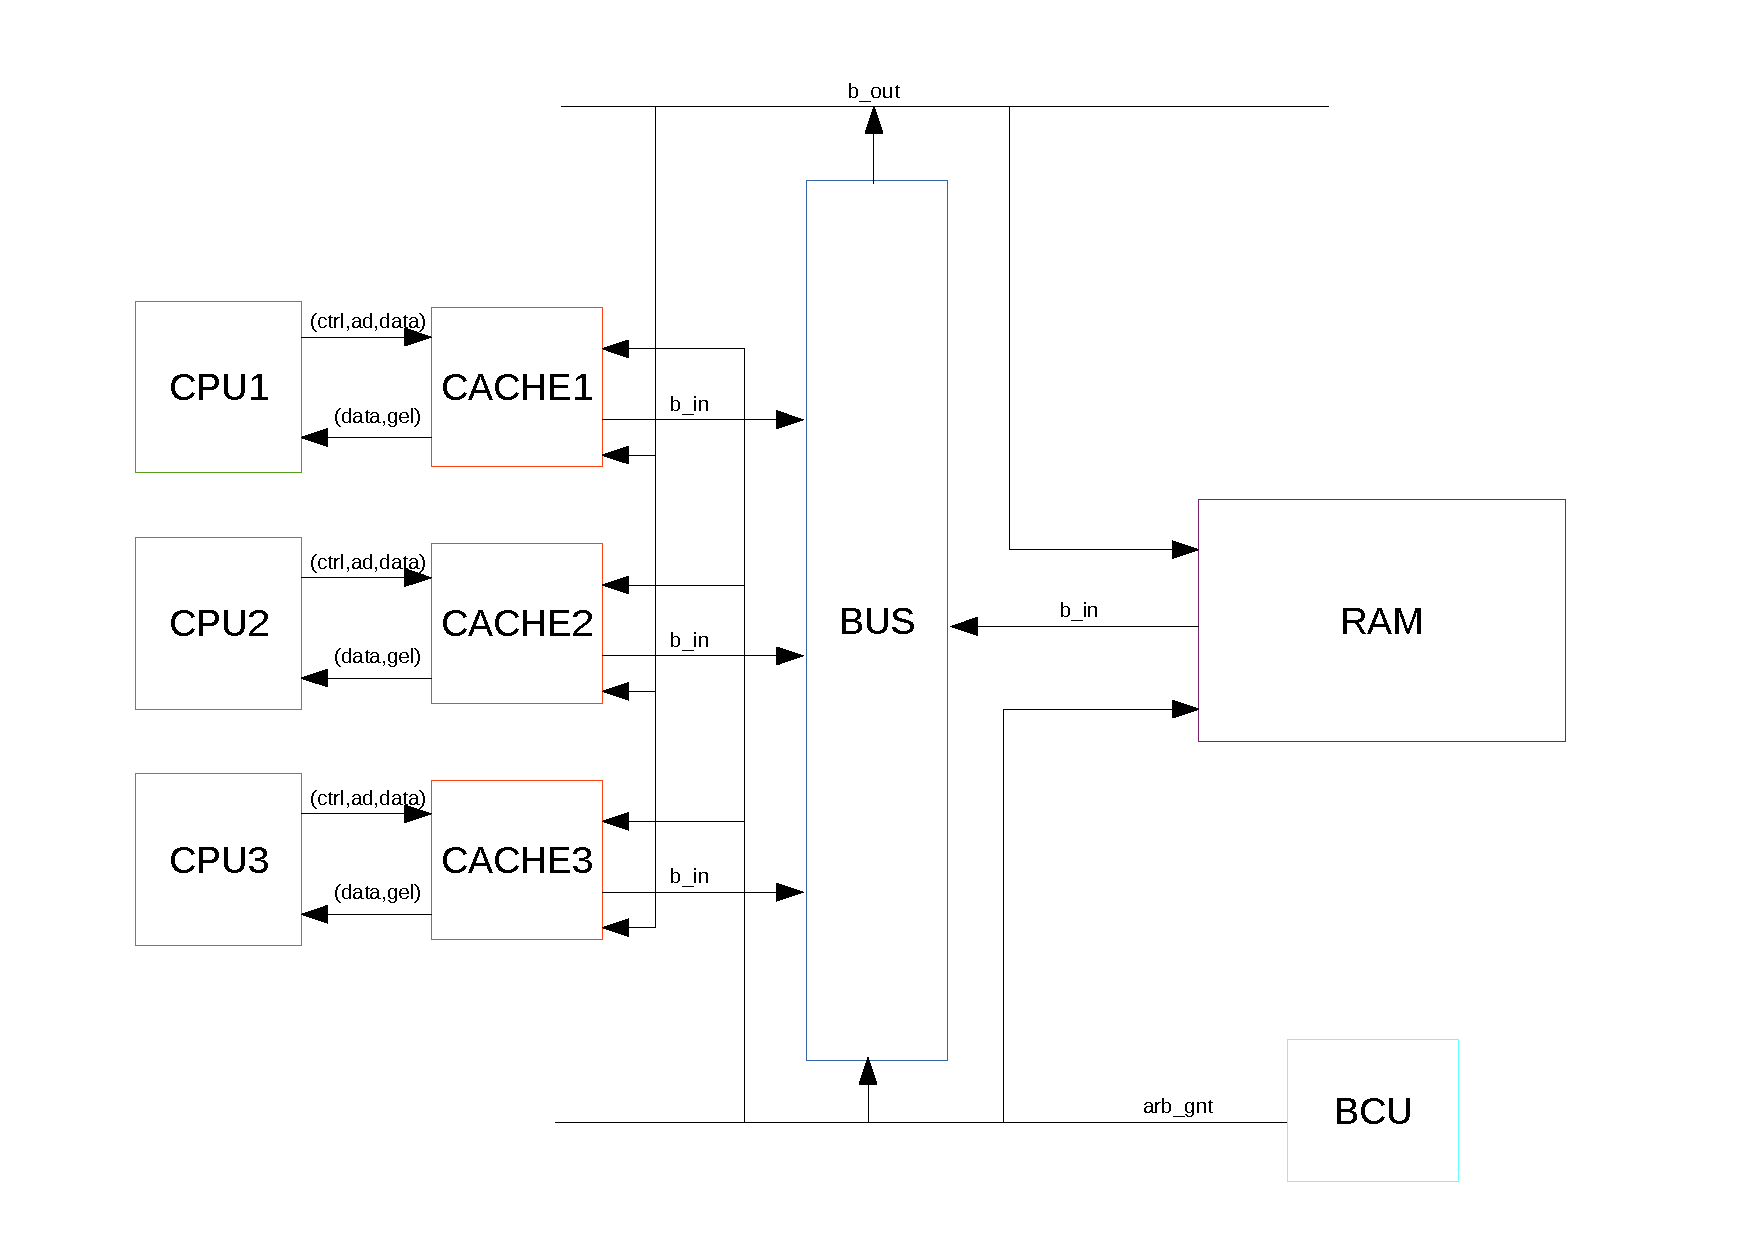
\includegraphics[scale=0.5]{images/archi.pdf}
\end{center}

\section{Bus}
Le bus a pour rôle de copier la nappe issue d'un processeur ou de la mémoire
vers la nappe de sortie du bus, selon le maître déterminé par le BCU (signal
\texttt{arb\_gnt}). Il doit validé la propriété suivante :
\begin{itemize}
  \item si une requête d'un processeur passe sur le bus, elle sera immédiatement
    suivie d'une réponse de la mémoire
\end{itemize}

\section{Processeur}
Le processeur prend en entrée un programme, ici simulé par les signaux suivants:
\begin{itemize}
  \item \texttt{op}: \textit{true} si écriture, lecture sinon;
  \item \texttt{valid}: \textit{true} si une instrution de type load ou store 
    est lue;
  \item \texttt{data\_in}: donnée à écrire si écriture;
  \item \texttt{ad}: adresse où lire/écrire en mémoire.
\end{itemize}
Il doit validé la propriété de vivacité suivante :
\begin{itemize}
  \item le processeur reviendra toujours à l'état non gelé
\end{itemize}
Dans l'implantation actuelle, cette propriété n'est pas vérifiée car le BCU
donne l'accès au bus toujours dans le même ordre. Une attribution par 
round-robin règlerait ce problème en supprimant les famines (voir code 
commenté du noeud bcu).

\section{Cache}
Le cache du processeur est modélisé sous la forme de l'automate suivant :
\begin{center}
\begin{tikzpicture}[->,>=stealth',shorten >=1pt,auto,node distance=4cm,
                    semithick]
  \tikzstyle{every state}=[fill=white,text=black]

  \node[state] (idle)                     {idle};
  \node[state] (rdmiss) [left of=idle]    {read\_miss};
  \node[state] (rdwait) [below of=rdmiss] {read\_wait};
  \node[state] (rdupd)  [below of=rdwait] {read\_update};
  \node[state] (wr)     [right of=idle]   {write};
  \node[state] (wrwait) [below of=wr]     {write\_wait};
  \path (idle)   edge [loop above] node {$(hit \bullet read)$}          (idle)
                 edge              node {$\overline{hit} \bullet read$} (rdmiss)
                 edge              node {$\overline{read}$}             (wr)
        (rdmiss) edge              node {$1$}                           (rdwait)
        (rdwait) edge [loop left]  node {$\overline{bus_{valid}}$}        (rdwait)
                 edge              node {$bus_{valid}$}                   (rdupd)
        (rdupd)  edge              node {$1$}                           (idle)
        (wr)     edge              node {$1$}                           (wrwait)
        (wrwait) edge              node {$bus_{valid}$}                   (idle)
                 edge [loop right] node {$\overline{bus_{valid}}$}        (wrwait);
        
\end{tikzpicture}
\end{center}
On suppose que si aucune requête n'est reçue, on reste dans l'état
\texttt{idle}. De plus, l'état \texttt{write} fait la mise à jour du cache en
cas de \textit{hit} et envoie la requête sur le bus dans tous les cas. L'état 
\texttt{idle} renvoie la valeur en cache en cas de \textit{hit} sur une lecture
en un cycle.

\end{document}
